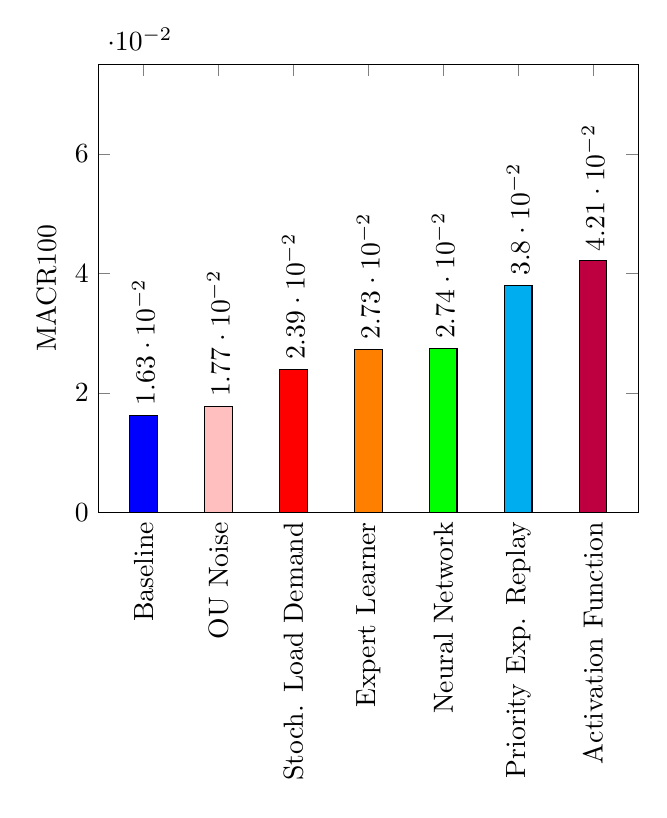
\begin{tikzpicture}
	\begin{axis}[
	    ylabel={MACR100},
	    symbolic x coords={Baseline,, OU Noise,, Stoch. Load Demand,, Expert Learner,, Neural Network,, Priority Exp. Replay,, Activation Function},
	    xtick = {Baseline, Neural Network, Activation Function, OU Noise, Priority Exp. Replay, Expert Learner, Stoch. Load Demand},
	    xticklabel style={rotate=90},
	    nodes near coords,
	    nodes near coords align={vertical},
	    every node near coord/.append style={rotate=90, anchor=west},
	    ymin=0, ymax=0.075
	    ]
	\addplot [ybar, fill=blue] coordinates {(Baseline, 0.0163)};
	\addplot [ybar, fill=green] coordinates {(Neural Network, 0.0274)};
	\addplot [ybar, fill=purple] coordinates {(Activation Function, 0.0421)};
	\addplot [ybar, fill=pink] coordinates {(OU Noise, 0.0177)};
	\addplot [ybar, fill=cyan] coordinates {(Priority Exp. Replay, 0.0380)};
	\addplot [ybar, fill=orange] coordinates {(Expert Learner, 0.0273)};
	\addplot [ybar, fill=red] coordinates {(Stoch. Load Demand, 0.0239)};
	%\legend{Baseline, Neural Network, Activation Function, OU Noise, Priority Experience Replay, Expert Learner, Stochastic Load Demand};
	\end{axis}
\end{tikzpicture}